\section{Introduction to Open Source Software: SigPy}
%=========================================================================================
\begin{frame}[fragile]{Why is linear operators abstraction convenient?}

\begin{block}<1->{Iterative image reconstruction 
		(e.g.~SENSE \footnote{Pruessmann KP, et al. SENSE: Sensitivity encoding for fast MRI. \textit{Magn Reson Med} (1999).}) solves:}
	{\large
	\begin{equation}
		\argmin_x \norm{y - \mathcal{F}_u S x}_2^2 + \lambda R(x)
	\end{equation}
	\begin{enumerate}[label*=\arabic*.]
		\item The unknown $x$ can go beyond 2D, and the forward operator can be extended.
		\item $S$ is the multiplication with coil sensitivity maps, 
			and $\mathcal{F}_u$ is the masked FFT or NUFFT.
		\item Its minimization often requires following operations:
			\begin{enumerate}[label*=\arabic*.]
				\item Gradient of the data consistency term: $S^* \mathcal{F}_u^{-1} (y - \mathcal{F}_u S x)$
				\item Adjoint of the regularization term: $R^H R$
			\end{enumerate}
	\end{enumerate}}
\end{block}

\begin{block}<2->{SigPy \footnote{Ong F. \url{https://github.com/mikgroup/sigpy.}} provides linear operators abstraction (e.g.~total variation)}
\begin{lstlisting}
>>> G = sp.linop.FiniteDifference([256, 256], axes=(-2, -1))
>>> y = G.H * G * x
\end{lstlisting}
\end{block}


\end{frame}

\begin{frame}[fragile]{Linear Operator Implementation}

\begin{block}{Linop is the parent class, and all basic child linear operators require:}
\begin{lstlisting}
    def __init__(self, oshape, ishape): # initialization
    def _apply(self, input): # apply the linop, e.g. G(x) or G * x
    def _adjoint_linop(self): # G.H
\end{lstlisting}
\end{block}

\begin{block}{e.g. Multiply, which is used for the coil sensitivity operator $S$}
	{\large
	\begin{itemize}
		\item [$\diamond$] Its \_apply function uses the multiply function in Python, \\
				e.g.~$I$ of shape $[256,256]$ * $C$ of shape $[4,256,256]$ outputs $R$ of $C$'s shape
		\vspace{1em}
		\item [$\diamond$] Its \_adjoint\_linop is then \\
				$\sum_{j=1}^{N_c} C_j^* \cdot I$, \\
				and is implemented as a \textbf{chain} of operators Reshape * Sum * Multiply
	\end{itemize}}
\end{block}

\end{frame}


\begin{frame}[fragile]{Example: Total Variation (TV)}

\begin{block}<1->{}
{\large
\begin{center}
	\begin{tabular}{ c | c | c }
		Given matrix A: $\begin{bmatrix}
			0 & 1 & 2 \\
			3 & 4 & 5 \\
			6 & 7 & 8
		\end{bmatrix}$ & 
		down roll by 1: $\begin{bmatrix}
			6 & 7 & 8 \\
			0 & 1 & 2 \\
			3 & 4 & 5
		\end{bmatrix}$ & 
		right roll by 1: $\begin{bmatrix}
			2 & 0 & 1 \\
			5 & 3 & 4 \\
			8 & 6 & 7
		\end{bmatrix}$ \\
	 	& 
\begin{lstlisting}
>>> np.roll(A, 1, axis=0)
\end{lstlisting} & 
\begin{lstlisting}
>>> np.roll(A, 1, axis=1)
\end{lstlisting}
	\end{tabular}
\end{center}}
\end{block}

\begin{block}<2->{Total variation \footnote{Rudin LI, et al. Nonlinear total variation based noise removal algorithms. \textit{Physica D} (1992).} is the subtraction 
		between the rolled and the input matrix.}
\begin{columns}
\begin{column}{0.55\textwidth}
	\begin{figure}
		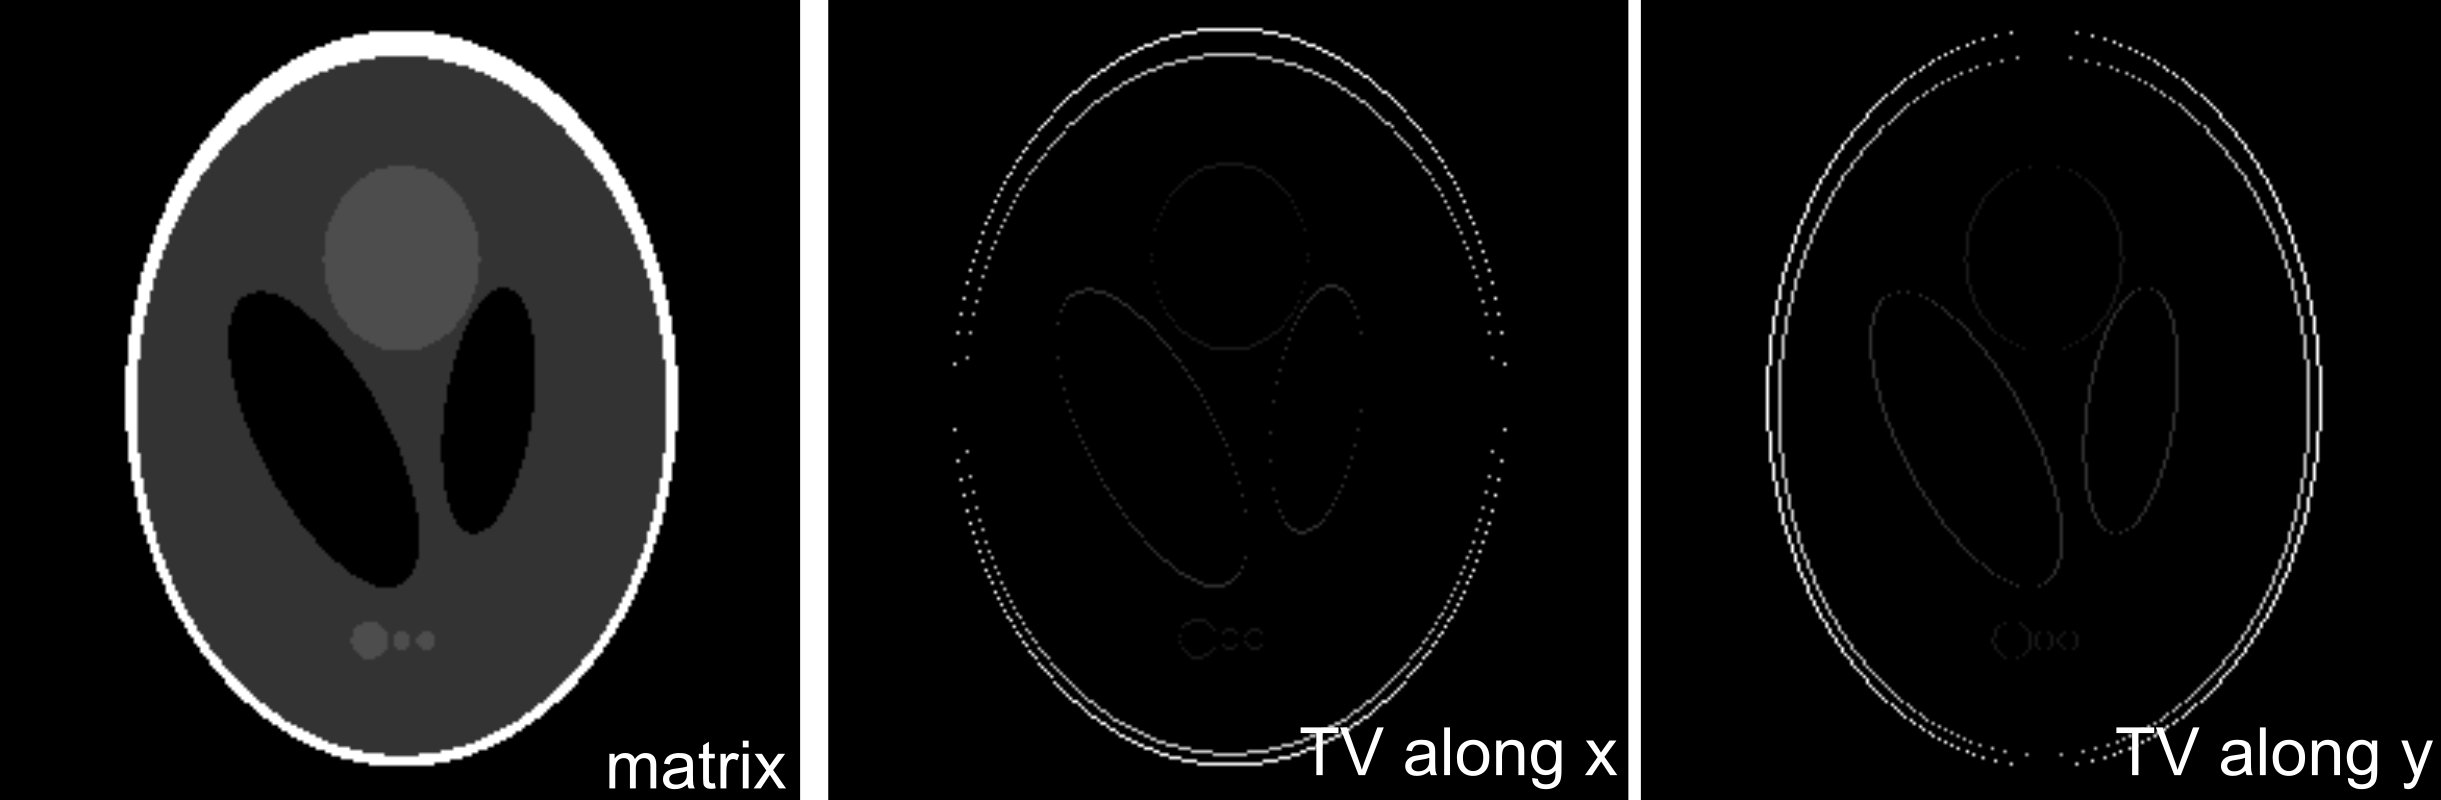
\includegraphics[width=0.9\columnwidth]{tv.png}
	\end{figure}
\end{column}

\begin{column}{0.45\textwidth}
\begin{lstlisting}
>>> I = shepp_logan((256, 256))
>>> G = linop.FiniteDifference(
		I.shape,
		axes=[-2, -1])
>>> y = G * x
\end{lstlisting}
\end{column}

\end{columns}
\end{block}

\end{frame}


\begin{frame}[fragile]{How to assert if the linop operator is correct?}

\begin{block}{Linear operator properties}
	{\large
	\begin{itemize}
		\item [$\diamond$] Unitary: $A^H * A * x = x \;\;\;$ and $\;\;\; <A*x,~y> = <x,~A^H*y>$
		\item [$\diamond$] Linearity: $A(a * x + y) = a * A(x) + A(y)$
	\end{itemize}}
\end{block}

\begin{block}{Routine Linop Test Functions}
\begin{lstlisting}
    shape = [256, 256]
    A = linop.FiniteDifference(shape)
    self.check_linop_adjoint(A)
    self.check_linop_normal(A)
    self.check_linop_linear(A)
\end{lstlisting}
\end{block}

\end{frame}

\subsection{Actual Practice: Locally Low Rank (LLR)}
%=================================================================================

\begin{frame}{Exploring Sparsity in Multi-Contrast Images 
	\footnote{Zhang T, et al. Accelerating parameter mapping with a locally low rank constraint
. \textit{Magn Reson Med} (2014).}}
	\begin{columns}
		\begin{column}{0.5\textwidth}
			\begin{figure}
				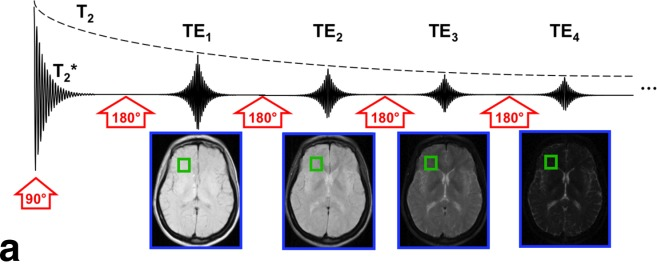
\includegraphics[width=\columnwidth]{llr_idea_a.png}
			\end{figure}
		\end{column}
		\begin{column}{0.5\textwidth}
			\begin{figure}
				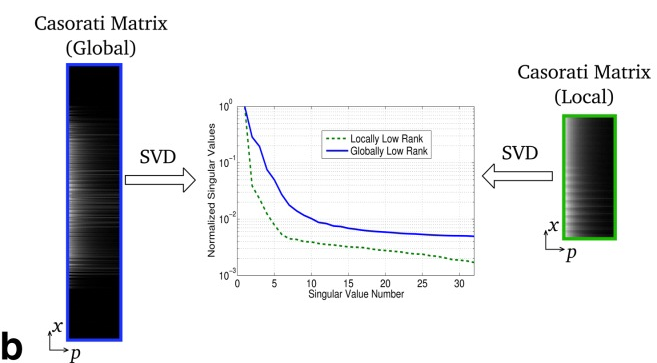
\includegraphics[width=\columnwidth]{llr_idea_b.png}
			\end{figure}
		\end{column}
	\end{columns}
\end{frame}

\begin{frame}{Locally Low Rank (LLR) Soft Thresholding Process}
	\begin{block}{LLR soft thresholding can be implemented as a proximal operator 
			\footnote{Beck A. First-order methods in optimization. \textit{SIAM} (2017).}.}
		\begin{figure}
			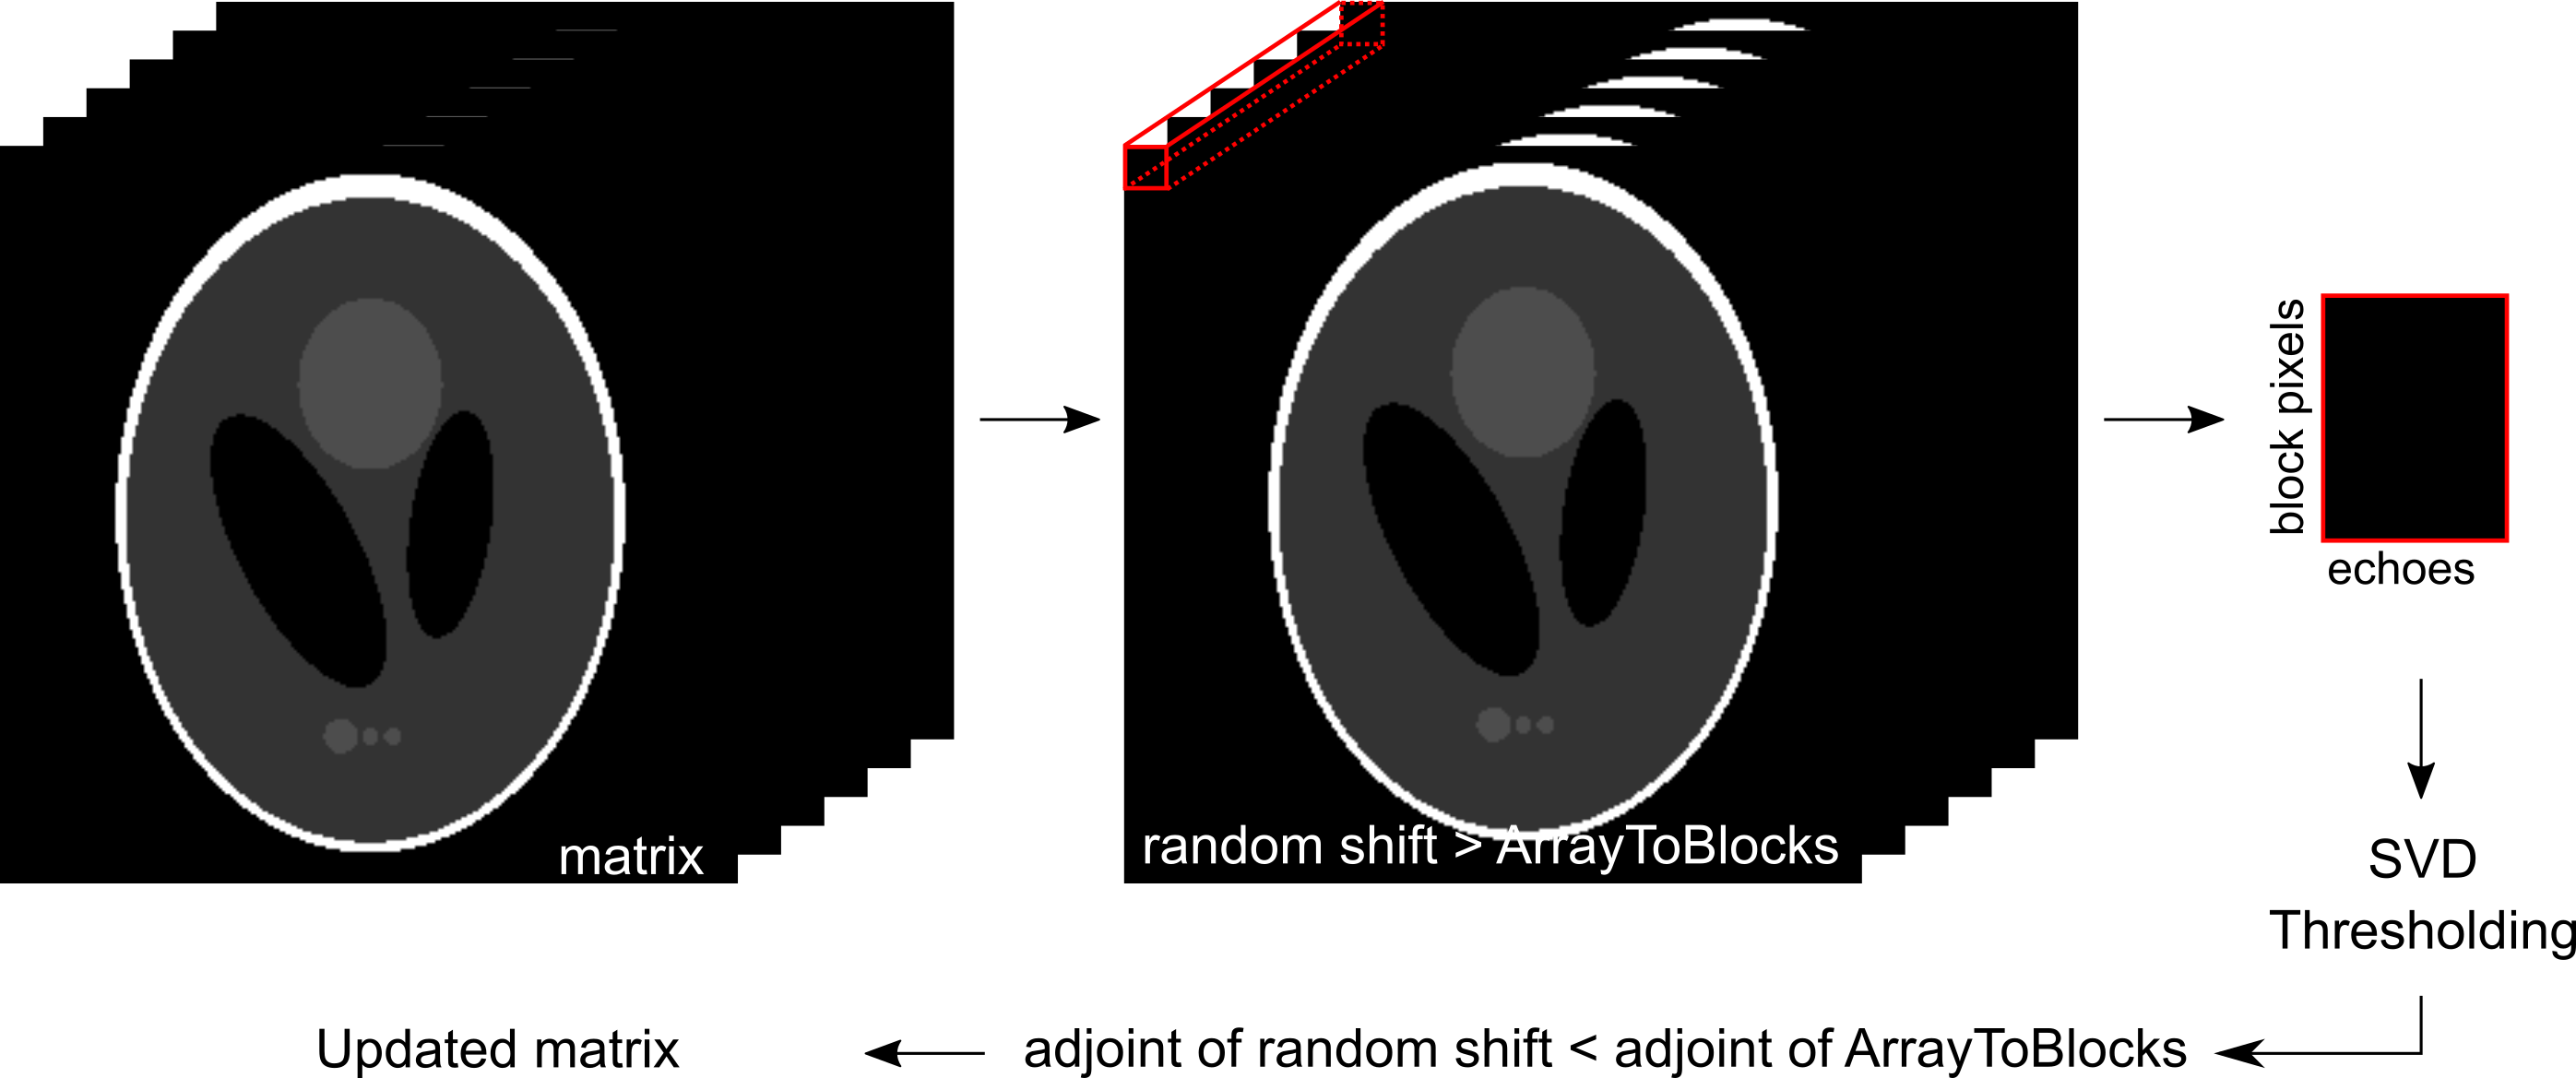
\includegraphics[width=0.8\textwidth]{llr_sthresh.png}
		\end{figure}
	\end{block}
\end{frame}


\begin{frame}[fragile]{Locally Low Rank (LLR) Soft Thresholding Implementation}
\begin{block}{Define all linops}
\begin{lstlisting}
def _linop_randshift(self):
    axes = [-2, -1]
    shift = [random.randint(0, self.blk_shape[s]) for s in axes]
    return linop.Circshift(self.shape, shift, axes)

RandShift = self._linop_randshift()
ATB = linop.ArrayToBlocks(shape, blk_shape, blk_strides)

def _linop_reshape(self):
    ...
    return R

Reshape = self._linop_reshape()
\end{lstlisting}
\end{block}

\end{frame}


\begin{frame}[fragile]{Locally Low Rank (LLR) Soft Thresholding Implementation}
\begin{block}{prox.LLRL1Reg}
\begin{lstlisting}
# forward
y1 = RandShift(input)
y2 = ATB(y1)
y3 = Reshape(y2)

# SVD soft thresholding
u, s, vh = np.linalg.svd(y3, full_matrices=False)
s_thresh = thresh.soft_thresh(self.lamda, s)
y4 = (u * s_thresh[..., None, :]) @ vh

# adjoint
y5 = Reshape.H(y4)
y6 = ATB.H(y5)
output = RandShift.H(y6)
\end{lstlisting}
\end{block}	
\end{frame}


\subsection{Actual Practice: LLR regularized Linear Subspace Reconstruction}
%=================================================================================

\begin{frame}{Linear Subspace Modeling Reduces the Number of Unknowns}
	\begin{block}<1->{}
	{\large
	\begin{equation}
		\argmin_x \norm{y - \mathcal{F}_u S x}_2^2 + \lambda \norm{\text{LLR}(x)}_1
	\end{equation}
	$x$ is multi-contrast images. However, the more contrast in the unknown requires longer reconstruction time.}
	\end{block}

	\begin{block}<2->{Linear subspace modeling 
		\footnote{Huang C, et al. T2 mapping from highly undersampled data by reconstruction of principal component coefficient maps using compressed sensing. \textit{Magn Reson Med} (2012).}$^,$
		\footnote{Tamir JI, et al. T2 shuffling: Sharp, multicontrast, volumetric fast spin-echo imaging. \textit{Magn Reson Med} (2017).}}
	{\large
	\begin{equation}
		\argmin_\alpha \norm{y - \mathcal{F}_u S \hat{U} \alpha}_2^2 + \lambda \norm{\text{LLR}(\alpha)}_1
	\end{equation}
	\begin{itemize}
		\item [$\diamond$] $\hat{U}$ is the truncated SVD of the simulated dictionary corresponding to the sequence protocol.
		\item [$\diamond$] $\alpha$ is the linear subspace coefficient maps
	\end{itemize}}
	\end{block}
\end{frame}

\begin{frame}{Solving LLR Regularized Linear Subspace Reconstruction}
Alternating Direction Method of Multipliers (ADMM) 
\footnote{Boyd S, et al. Distributed optimization and statistical learning via the alternating direction method of multipliers. \textit{Found Trends Mach Learn} (2010).}

\begin{equation}
\begin{aligned}
	\text{minimize}~&l(x) + g(z) \\
	\text{subject to}~&x - z =0
\end{aligned}
\end{equation}
$l(x)$ is the data consistency term, and $g(z)$ is the regularization.

\vspace{1em}

\begin{equation}
\begin{aligned}
	x^{k+1} &:= \argmin_x l(x) + (\rho/2) \norm{x - x^k + u^k}_2^2 \\
	z^{k+1} &:= S_{\lambda/\rho} (x^{k+1} + u^{k}) \\
	u^{k+1} &:= u^k + x^{k+1} - z^{k+1}
\end{aligned}
\end{equation}

\end{frame}
